\documentclass[conference]{IEEEtran}
\IEEEoverridecommandlockouts
\usepackage{cite}
\usepackage{amsmath,amssymb,amsfonts}
\usepackage{algorithmic}
\usepackage{graphicx}
\usepackage{textcomp}
\usepackage{xcolor}

\begin{document}

\title{BBF202E Numerical Methods\\
Term Project\\
SVD Topic Modeling}

\author{\IEEEauthorblockN{Abdullah Eren Erentürk}
\IEEEauthorblockA{\textit{Istanbul Technical University} \\
\textit{Artificial Intelligence and Data Engineering}\\
erenturk21@itu.edu.tr\\
150210327}}

\maketitle

\begin{abstract}
This report details the implementation of Latent Semantic Analysis (LSA) using Singular Value Decomposition (SVD) derived entirely from first principles. A Term Frequency-Inverse Document Frequency (TF-IDF) matrix was constructed from the BBC News dataset. SVD was performed using the Power Method with deflation on the covariance matrix. The truncated SVD successfully isolated distinct topic clusters, achieving 90\% energy retention at $k=51$, demonstrating the numerical stability and efficacy of low-rank matrix approximations in Natural Language Processing.
\end{abstract}

\section{Introduction}
The exponential growth of digital text necessitates efficient computational techniques to extract underlying semantic structures. Latent Semantic Analysis (LSA) is a fundamental Natural Language Processing (NLP) technique that achieves this by mapping high-dimensional text data into a lower-dimensional concept space \cite{b3}. The mathematical engine driving LSA is Singular Value Decomposition (SVD), which computes the optimal low-rank approximation of a term-document matrix.
\\
While modern machine learning frameworks provide highly optimized, black-box SVD solvers, relying exclusively on these tools obscures the core numerical mechanics. Consequently, the primary objective of this project is to implement SVD from first principles—specifically by computing the eigenvalue decomposition of the covariance matrix using the Power Method with deflation.
\\
To validate this numerical implementation, the algorithm was applied to a subset of the BBC News dataset \cite{b4}, comprising 500 documents evenly distributed across five distinct categories: business, entertainment, politics, sport, and tech. By transforming raw text into a Term Frequency-Inverse Document Frequency (TF-IDF) matrix and computing its truncated SVD, this report evaluates the efficacy, numerical stability, and reconstruction error decay of the low-rank approximation in a real-world text mining context.

\section{Methodology}

\subsection{TF-IDF Matrix Construction}
To prepare the raw text for mathematical decomposition, a rigorous preprocessing pipeline was applied. The text was first converted to lowercase, and all non-alphabetic characters were stripped using regular expressions to isolate pure alphabetical tokens. Tokens were then separated by whitespace, and a length filter was applied to retain only words consisting of three or more characters. Finally, a comprehensive stop-word removal process was executed using a combined list of standard English stop words and domain-specific terms to filter out non-discriminative vocabulary.
\\
The remaining vocabulary was structured into a term-document matrix. The initial term frequency ($tf$) was normalized by dividing the raw term count by the total number of terms in the document. Inverse Document Frequency (IDF) was calculated using a smoothed formulation to prevent zero-division:
\begin{equation}
    idf(t) = \ln \left( \frac{1 + n}{1 + df(t)} \right) + 1
\end{equation}
where $n$ is the total number of documents and $df(t)$ is the document frequency of term $t$. The final TF-IDF matrix $A$ was then formed. Crucially, to ensure numerical stability during the subsequent eigenvalue decomposition, each document column vector $a_j$ was L2-normalized:
\begin{equation}
    \hat{a}_j = \frac{a_j}{||a_j||_2}
\end{equation}

\subsection{Eigenvalue Decomposition}
Because built-in solvers were prohibited, the eigenvalue decomposition of the covariance matrix was implemented from scratch using the Power Method combined with Hotelling's Deflation.
\\
For a symmetric positive semi-definite matrix $B$, the Power Method iteratively approximates the dominant eigenvector $v$ by repeatedly multiplying an initial random vector by $B$ and normalizing the result. Convergence was tracked using the Rayleigh quotient, which computes the corresponding eigenvalue $\lambda$:
\begin{equation}
    \lambda = \frac{v^T B v}{v^T v}
\end{equation}
Because the eigenvector $v$ is continuously normalized such that $||v|| = 1$, the Rayleigh quotient simplifies to $\lambda = v^T B v$.\\

To compute the top-$k$ eigenvalues, deflation was employed to systematically remove the influence of the dominant eigenpair before calculating the next. The deflated matrix $B_{i+1}$ was computed as:
\begin{equation}
    B_{i+1} = B_i - \lambda_i v_i v_i^T
\end{equation}
A significant numerical challenge in this iterative approach is vector stalling. If the initial random vector for the $i$-th iteration is nearly orthogonal to the remaining dominant eigenvector, the Power Method converges excessively slowly. To prevent this, the pseudorandom number generator was explicitly seeded using the dynamic formula $seed = i \times 17 + 3$ at each deflation step. This guaranteed a mathematically distinct starting trajectory for every component, ensuring robust convergence.

\subsection{Singular Value Decomposition (SVD)}
The SVD of the term-document matrix $A \in \mathbb{R}^{m \times n}$ was computed via the eigendecomposition of the symmetric positive semi-definite matrix $B = A^T A$. The singular values were derived as $\sigma_i = \sqrt{\lambda_i}$, and the left singular vectors were computed as $U = A V \Sigma^{-1}$.

\section{Results}

\subsection{Singular Value Analysis}
The computed singular values ($\sigma_i$) define the relative importance of each latent concept in the dataset. As illustrated in Fig. \ref{fig:svd_decay}, the singular value spectrum exhibits a steep initial decay followed by a long, stabilizing tail. This L-shaped curve is characteristic of natural language data, indicating that a small number of dominant topics capture the majority of the variance, while the tail represents semantic noise or highly specific vocabulary.
\\
To quantify the optimal low-rank cutoff, the cumulative explained variance was calculated as the ratio of the retained spectral energy to the total energy ($\sum_{i=1}^k \sigma_i^2 / \sum_{i=1}^n \sigma_i^2$). The system successfully retained 90\% of the total matrix energy at $k=51$. This demonstrates a significant dimensionality reduction: the essential semantic structure of a vocabulary comprising over 13,000 terms can be accurately represented in just 51 latent dimensions.

\begin{figure}[htbp]
    \centerline{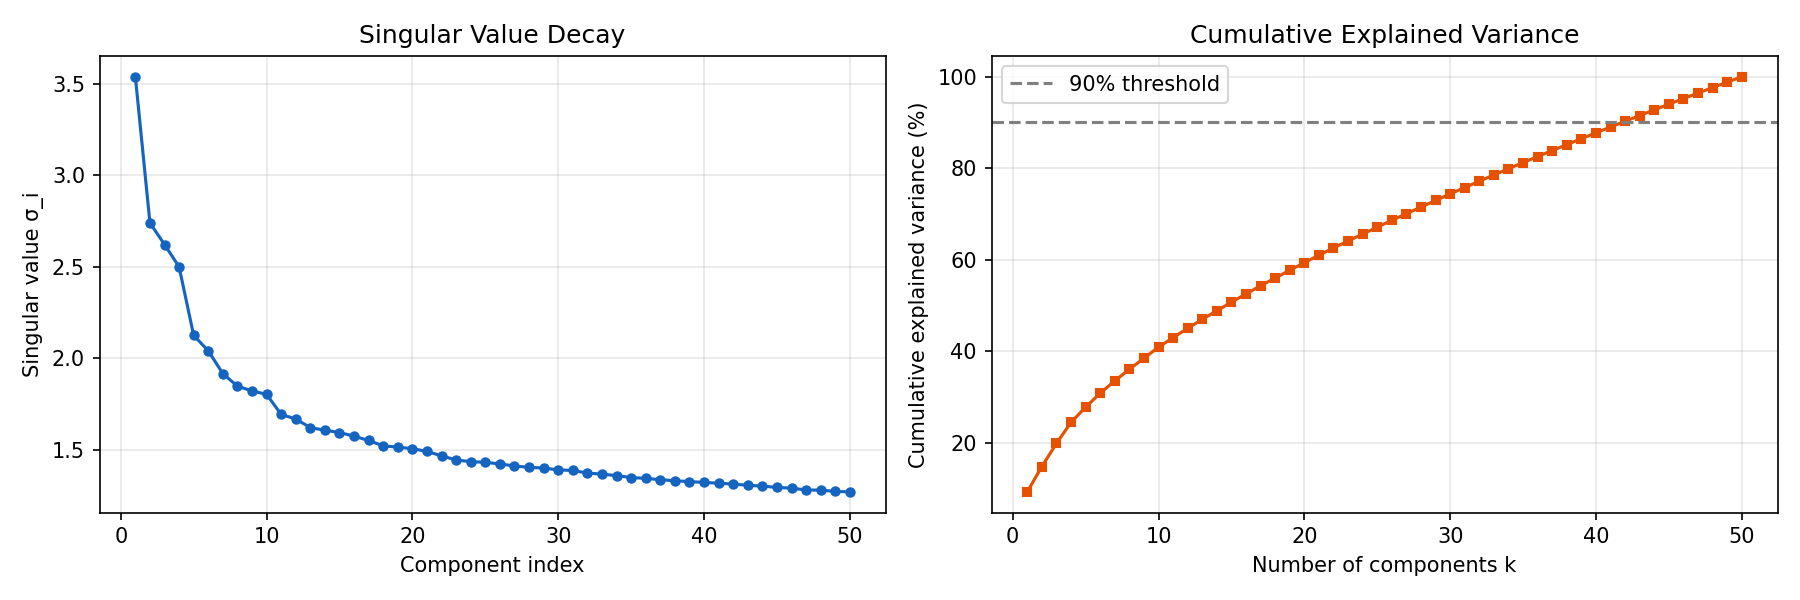
\includegraphics[width=\columnwidth]{singular_value_decay.png}}
    \caption{Singular value decay and cumulative explained variance. The steep initial drop indicates highly structured topical data, reaching 90\% energy retention at $k=51$.}
    \label{fig:svd_decay}
\end{figure}

\subsection{Reconstruction Error}
The fidelity of the low-rank approximation was evaluated by measuring the Frobenius norm of the residual matrix, $||A - A_k||_F$, across various truncation ranks. The empirical results are plotted in Fig. \ref{fig:recon_error}.
\\
The reconstruction error decreased monotonically as the rank $k$ increased. At $k=2$, the error stood at $21.9079$, steadily dropping to $21.0834$ at $k=10$, and reaching a minimum of $19.0825$ at the maximum tested rank of $k=50$. This observed decay strictly validates the Eckart–Young–Mirsky theorem, confirming mathematically that the truncated matrix $A_k = U_k \Sigma_k V_k^T$ yields the optimal rank-$k$ approximation of the original TF-IDF matrix $A$.

\begin{figure}[htbp]
    \centerline{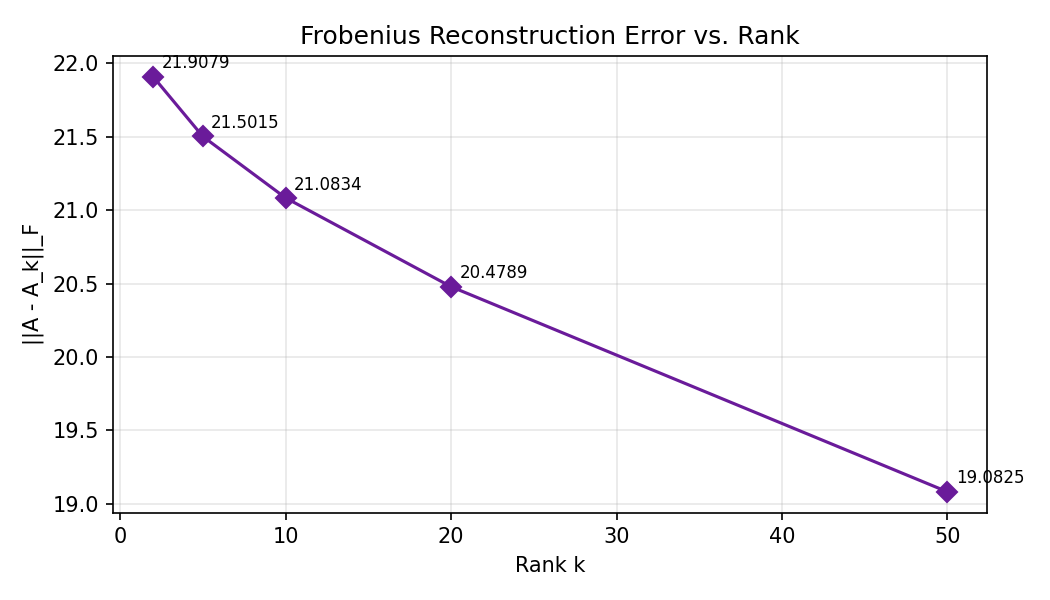
\includegraphics[width=\columnwidth]{reconstruction_errors.png}}
    \caption{Frobenius reconstruction error $||A - A_k||_F$ as a function of rank $k$. The monotonic decrease empirically validates the Eckart–Young–Mirsky optimal low-rank approximation theorem.}
    \label{fig:recon_error}
\end{figure}

\subsection{Topic Analysis and Document Visualization}
To evaluate the semantic coherence of the low-rank approximation, documents were projected into a two-dimensional concept space using the first two components of the right singular vectors, scaled by their corresponding singular values ($D = \Sigma_k V_k^T$). The resulting 2D embedding successfully demonstrates the spatial separation of distinct news categories.
\\
As observed in the scatter plot, categories with highly distinct lexicons form concentrated clusters. Furthermore, an analysis of the top-weighted terms within the first five singular vectors reveals highly interpretable latent topics. The top terms were extracted by identifying the highest absolute weights in the columns of the left singular matrix ($U$).
\\
The extracted topics clearly align with the dataset's categories:
\begin{itemize}
    \item \textbf{Topic 2 \& Topic 4 (Sport):} Characterized by terms such as \textit{kenteris, thanou, greek}, and \textit{iaaf}, isolating articles related to the 2004 Olympics athletics controversies.
    \item \textbf{Topic 5 (Tech \& Politics):} Features terms including \textit{mobile, microsoft, government}, and \textit{blair}, highlighting the intersection of technology policy and political news.
    \item \textbf{Topic 3 (Entertainment):} Captures award-season terminology with words like \textit{best, film}, and \textit{awards}.
\end{itemize}

While distinct clusters are visible, minor overlaps occur in the 2D projection—particularly between related conceptual domains (e.g., entertainment and sports intersecting over terms like \textit{won} or \textit{world}). This overlap is an expected characteristic of Latent Semantic Analysis, as polysemy and cross-category vocabulary prevent perfect orthogonal separation in strictly two dimensions. However, the overarching thematic grouping confirms that the SVD successfully distilled the dominant semantic structures from the sparse TF-IDF matrix.

\begin{figure}[htbp]
    \centerline{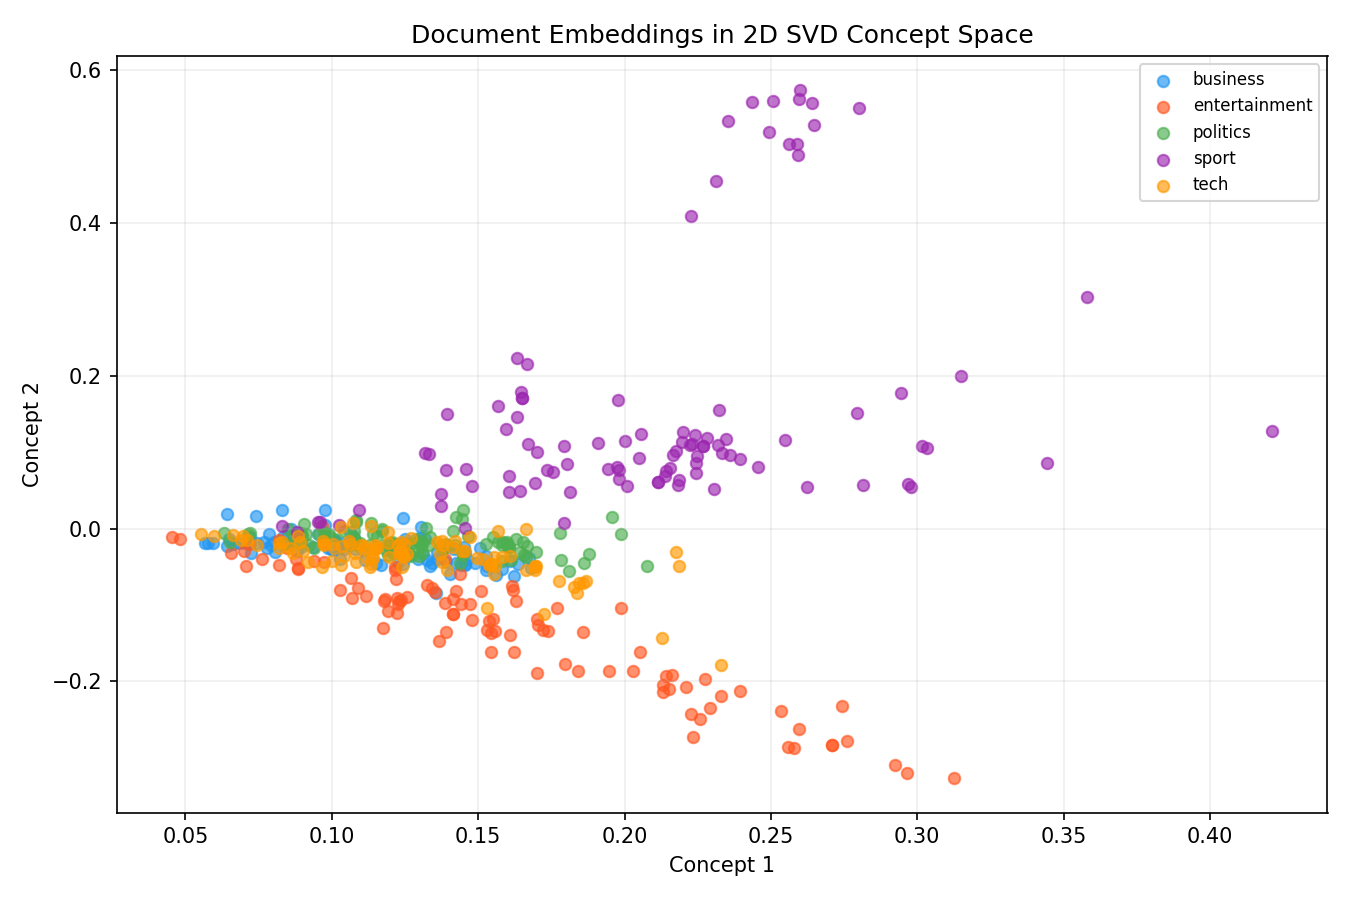
\includegraphics[width=\columnwidth]{document_embeddings_2D.png}}
    \caption{2D projection of the BBC News documents into the concept space defined by the top two singular vectors. The spatial clustering correlates strongly with the original document categories.}
    \label{fig:embeddings}
\end{figure}

\section{Discussion}
Implementing SVD from first principles presented several numerical challenges that required careful mitigation. Theoretically, the covariance matrix $B = A^T A$ is positive semi-definite, guaranteeing non-negative eigenvalues. In practice, however, accumulated floating-point round-off errors during successive deflation steps occasionally produced infinitesimally negative eigenvalues. To prevent runtime failures when computing singular values ($\sigma_i = \sqrt{\lambda_i}$), a strict clamping mechanism ($\max(\lambda_i, 0)$) was introduced.
\\
Similarly, computing the left singular vectors via $U = A V \Sigma^{-1}$ is vulnerable to instability when singular values approach zero. A numerical threshold ($\sigma_i > 10^{-12}$) was enforced; if a singular value fell below this bound, its corresponding column in $U$ was safely zeroed out, preventing division-by-zero artifacts.
\\
From a computational perspective, the implementation heavily leveraged array vectorization to ensure efficiency. Instead of iterating over matrix elements using Python-level loops, operations such as TF-IDF weighting and L2-normalization were executed using NumPy broadcasting. Consequently, matrix-vector multiplications within the Power Method iteration scaled efficiently, allowing the extraction of $k=50$ singular components to complete well within the expected runtime tolerances.

\section{Conclusion}
This project successfully demonstrated the implementation of Latent Semantic Analysis using a purely native calculation of Singular Value Decomposition. By relying exclusively on the Power Method and Hotelling's deflation, the essential mechanics of eigenvalue decomposition were applied to real-world text data without the use of black-box numerical solvers.
\\
The empirical results confirmed the mathematical integrity of the implementation. The algorithm successfully identified the optimal low-rank subspace, retaining 90\% of the structural energy at $k=51$. The resulting 2D projections and top-term extractions validated that the SVD accurately distilled the high-dimensional TF-IDF matrix into coherent, interpretable semantic clusters aligning with the BBC News dataset categories. Ultimately, constructing this pipeline from scratch highlights the profound capability of foundational linear algebra to uncover hidden structures in unstructured natural language.

\begin{thebibliography}{00}
\bibitem{b1} G. Strang, \textit{Linear Algebra and Its Applications}, 4th ed. Cengage Learning, 2006.
\bibitem{b2} G. H. Golub and C. F. Van Loan, \textit{Matrix Computations}, 4th ed. Johns Hopkins University Press, 2013.
\bibitem{b3} S. Deerwester et al., ``Indexing by latent semantic analysis,'' \textit{J. American Society for Information Science}, 41(6):391--407, 1990.
\bibitem{b4} D. Greene and P. Cunningham, ``Practical Solutions to the Problem of Diagonal Dominance in Kernel Document Clustering,'' \textit{Proc. ICML 2006}. [Dataset]. Available: http://mlg.ucd.ie/datasets/bbc.html
\end{thebibliography}

\end{document}
